\documentclass[tikz,border=10pt]{standalone}
\usetikzlibrary{calc, arrows.meta, shapes.geometric}

\begin{document}
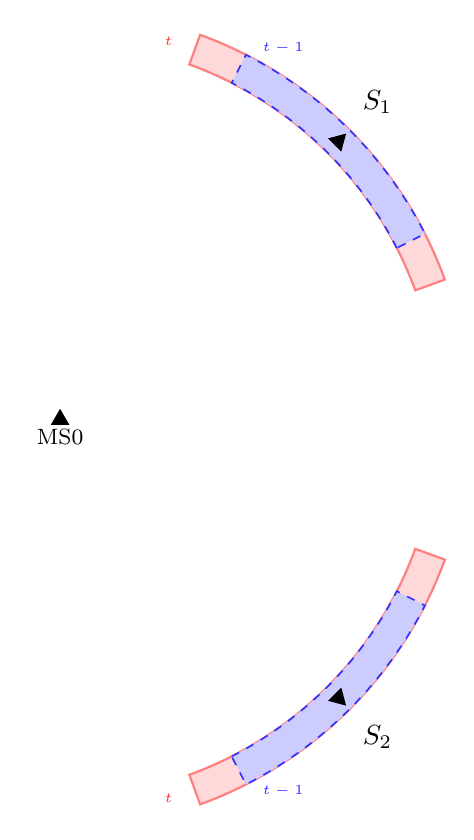
\begin{tikzpicture}[>=Stealth, font=\small]

    % --- Paramètres ---
    \def\R{5}                % Distance radiale
    \def\angS{45}            % Angle de la formation
    \def\dR{0.2}             % Épaisseur réduite et identique
    
    \def\spreadT{25}         % Longueur réduite à l'instant t
    \def\spreadTminus{18}    % Longueur réduite à l'instant t-1

    \coordinate (MS0) at (0,0);
    \coordinate (S1_pos) at (\angS:\R);
    \coordinate (S2_pos) at (-\angS:\R);

    % --- Styles de couleurs ---
    \tikzstyle{arc_t_minus} = [fill=blue!20, draw=blue!80, dashed, line width=0.6pt]
    \tikzstyle{arc_t} = [fill=red!15, draw=red!50, line width=0.8pt]

    % --- SCOUT S1 (Haut) ---
    % Arc t (rouge adouci)
    \fill[arc_t] (\angS-\spreadT:\R-\dR) arc (\angS-\spreadT:\angS+\spreadT:\R-\dR) -- (\angS+\spreadT:\R+\dR) arc (\angS+\spreadT:\angS-\spreadT:\R+\dR) -- cycle;
    % Arc t-1 (bleu)
    \fill[arc_t_minus] (\angS-\spreadTminus:\R-\dR) arc (\angS-\spreadTminus:\angS+\spreadTminus:\R-\dR) -- (\angS+\spreadTminus:\R+\dR) arc (\angS+\spreadTminus:\angS-\spreadTminus:\R+\dR) -- cycle;

    % Labels S1
    \node[red!80, font=\tiny\bfseries] at (\angS+\spreadT+4:\R) {$t$};
    \node[blue!80, font=\tiny\bfseries] at (\angS+\spreadTminus-4:\R+0.5) {$t-1$};
    \node[font=\bfseries] at (\angS:\R+0.7) {$S_1$};

    % --- SCOUT S2 (Bas) ---
    % Arc t
    \fill[arc_t] (-\angS-\spreadT:\R-\dR) arc (-\angS-\spreadT:-\angS+\spreadT:\R-\dR) -- (-\angS+\spreadT:\R+\dR) arc (-\angS+\spreadT:-\angS-\spreadT:\R+\dR) -- cycle;
    % Arc t-1
    \fill[arc_t_minus] (-\angS-\spreadTminus:\R-\dR) arc (-\angS-\spreadTminus:-\angS+\spreadTminus:\R-\dR) -- (-\angS+\spreadTminus:\R+\dR) arc (-\angS+\spreadTminus:-\angS-\spreadTminus:\R+\dR) -- cycle;

    % Labels S2
    \node[red!80, font=\tiny\bfseries] at (-\angS-\spreadT-4:\R) {$t$};
    \node[blue!80, font=\tiny\bfseries] at (-\angS-\spreadTminus+4:\R+0.5) {$t-1$};
    \node[font=\bfseries] at (-\angS:\R+0.7) {$S_2$};

    % --- Bateaux (Triangles) ---
    \node[draw, fill=black, regular polygon, regular polygon sides=3, inner sep=1pt, minimum size=7pt] at (MS0) {};
    \node[below, font=\footnotesize] at (MS0) {MS0};
    
    \node[draw, fill=black, regular polygon, regular polygon sides=3, inner sep=1pt, minimum size=7pt, rotate=\angS-90] at (S1_pos) {};
    \node[draw, fill=black, regular polygon, regular polygon sides=3, inner sep=1pt, minimum size=7pt, rotate=-\angS-90] at (S2_pos) {};

\end{tikzpicture}
\end{document}